\newpage
\hypertarget{m2tvis}{}
\subsection{Vis model to tree}
\visHeader

\begin{itemize}

\item[$\blacktriangleright$] Even though they've been built, our unparsed files are still empty. This second rule pair will convert model-to-text

\item[$\blacktriangleright$] We'll to model-to-tree using TGG, but tree-to-text using ANTLR, our unparser pair. But, remember the benefits of TGGs? If we
establish one direction, we should be able to get the second for free, right? Copy and rename \texttt{tree.xmi\_fwd.xmi} to \texttt{model}.

\item[$\blacktriangleright$] Then, re-open \texttt{TGG.main} and edit line 34 from \texttt{target} to \texttt{model}.
	
\item[$\blacktriangleright$] Refresh your \emph{instances} folder. Open \texttt{model.xmi\_bwd.xmi}. Perfect! This is how our output hierarchy looks like. Our
main folder, with two shelf folders. Expanding \texttt{english}, for example, it has one file. that file then has an dictionary node, as well as
one for title, author, and each entry.

\item[$\blacktriangleright$] Compare it to our original \texttt{tree.xmi}. It should be similar! But there IS some information missing - let's update our TGG.

\item[$\blacktriangleright$] Open \texttt{NodeToDictionaryRule} and update as depicted below (via attribute constraint)

\begin{figure}[htp]
\begin{center}
  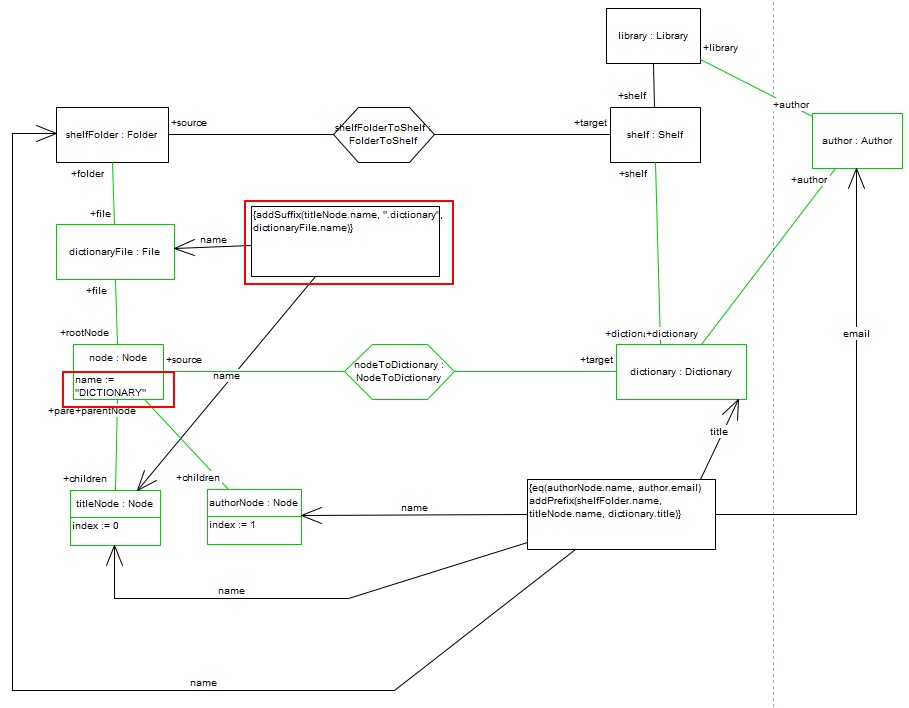
\includegraphics[width=\textwidth]{ea_updateNodeToDictionary}
  \caption{updated NodeToDictionary}
  \label{ea:NodeToDictionary_updated}
\end{center}
\end{figure}

\item[$\blacktriangleright$] Switch back to eclipse and run TGG main again to confirm the change. It worked!

\item[$\blacktriangleright$] Similarly, open \texttt{ForAllEntry} in EA and update like so:

\begin{figure}[htp]
\begin{center}
  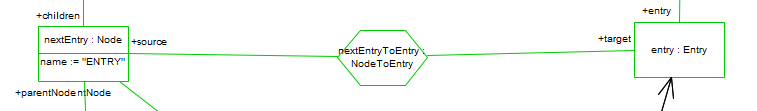
\includegraphics[width=\textwidth]{ea_updateForAllEntry}
  \caption{updated ForAllEntry}
  \label{ea:ForAllEntry_updated}
\end{center}
\end{figure}

\item[$\blacktriangleright$] Final challenge is getting the right name for the \texttt{File}. We'll need to use a \texttt{Moca.Util} method invocation here.
All of these changes make sense in THIS section as we're refining/defining for the backwards transformation. Should resemble (with the possible exception of
order) the original \texttt{tree.xmi} very closely.

\end{itemize}